\documentclass{hw}
\title{Programming Assignment 1:\\ Implementing Lexical Analysis}

\usepackage{fancyvrb}
\usepackage{pervasives}
\usepackage{tikz}
\usetikzlibrary{positioning}

\begin{document}
\maketitle

\section{Metadata}\label{sec:metadata}
% The fully qualified class name of your main program and any other
% instructions needed to run the program.
Our main executable is implemented in \texttt{mjw297.Main.java} which is found
in the \texttt{src/mjw297} directory. To build our executable, simply run
\texttt{make src}. This will use \texttt{jflex}, \texttt{cup}, and
\texttt{javac} and build all of our code. Our Makefile depends only on
\texttt{javac}; all our dependencies, including \texttt{jflex} and
\texttt{cup}, are packaged in the \texttt{lib} directory.  Note that we enabled
warnings when compiling with \texttt{javac} and that the lexer generated by
JFlex and the \texttt{Sym} class generated by CUP both generate warnings. These
warnings will be seen when building our code.  None of our own code generates
warnings. In the rare event that compilation fails, we have also packaged our
compiled bytecode and generated lexer code with our submission.

Invoking \texttt{mjw297.Main} can be tricky because you have to include the
JARs inside of our \texttt{lib} directory in your classpath. To run our lexer,
we recommend you use the \texttt{xic} script which invokes \texttt{mjw297.Main}
with everything configured properly. In summary, perform the following:

\begin{center}
\begin{BVerbatim}
make src
./xic --lex <xi_file.xi>...
\end{BVerbatim}
\end{center}

\section{Summary}\label{sec:summary}
In this programming assignment, we implemented a lexer in Java for the Xi
programming language using the JFlex lexer generator and CUP parser generator.
Our major design decisions involve the design of symbol and exception classes,
the choice of language and libraries, and the lexing of a few nefarious Xi
programs. The most challenging aspect of the assignment was the handling of
non-printable characters inside of comments, strings, and characters. For
example, the form feed character `\verb$\f$' is a non-printable character that
is difficult to lex correctly in various contexts. There are no known problems
with our implementation.

\section{Specification}\label{sec:specification}
In this section, we make explicit our interpretation of the Xi language
specification and discuss various language extensions we have implemented.

\subsection{Line Endings and Whitespace}
The Xi language specification is ambiguous about the definition of a line
terminator, referring to it only informally as a ``newline''. We define a line
terminator to be a carriage return `\verb$\r$', a newline `\verb$\n$', or both
`\verb$\r\n$'. If a `\verb$\r\n$' is present, it is counted as a single
newline. This definition of line terminators is consistent with the Java
Language
Specification\footnote{\url{https://docs.oracle.com/javase/specs/jls/se8/html/jls-3.html\#jls-3.4}}.
Similarly we define whitespace to be any of `\verb$\r$', `\verb$\n$',
`\verb$\r\n$', `\verb$ $', `\verb$\t$', `\verb$\f$'. This is also consistent with
the Java Language
Specification\footnote{\url{https://docs.oracle.com/javase/specs/jls/se8/html/jls-3.html\#jls-3.6}}.

\subsection{Comments}
The Xi language specification states that a comment is \texttt{//} followed by
any sequence of characters until a newline character. We interpret a newline
character to be any line terminator as defined above. We have also made a small
revision and allow comments to be terminated by the end of a file as described
in \secref{design}.

\subsection{Characters in Comments, Strings, and Characters}
Xi input files are UTF-8 encoded, though keywords and identifiers are made up
of only ASCII characters. This leads to the question of what characters are
allowed inside of comments, strings, and character literals. We allow any
character that is not a line terminator, including exotic Unicode characters,
to appear in a comment, string, or character literal. Allowing exotic
characters simplifies the lexer and provides a bit of flexibility to
Xi programmers.

\subsection{Hex and Unicode Escape Sequences}
The programming assignment mandates that we support hex escape sequences inside
of string and character literals. For example, the string \verb$"\x64"$ is
lexed into the string \texttt{"d"}. The programming assignment is ambiguous
about the format of the hex escape sequences. We support only fixed width
two-digit hex escape sequences.
%
In addition to hex escape sequences, we have also added Unicode escape
sequences of the form:
\begin{center}
  \verb$\u[a-fA-F0-9][a-fA-F0-9][a-fA-F0-9][a-fA-F0-9]$
\end{center}
For example, the string \verb$"\u0064"$ lexes to \texttt{"d"}.

\subsection{Escape Characters}
The Xi language specification says to support a ``reasonable'' set of character
escapes. We have elected to support \verb$\t$, \verb$\b$, \verb$\n$, \verb$\r$,
\verb$\f$, \verb$\'$, \verb$\"$, and \verb$\\$. These are also the set of
non-printable characters that our compiler pretty prints when run with the
\texttt{--lex} flag. For example the Xi string \verb$"\n"$ is printed as
\verb$\n$ rather than a literal newline. All other non-printable characters are
printed as hex escaped sequences.

\subsection{Non-Line Terminating Whitespace}
Certain whitespace character are not Xi line terminators but are often
considered in other contexts to be line terminators. For example, \verb$\f$,
\verb$\u2028$, and \verb$\u2029$ are considered by JFlex to be line
terminators.  This leads to an inconsistency in the row numbers our lexer
reports. The number of lines reported by JFlex is not consistent with the
number of lines terminated by a Xi line terminator. Since these whitespace
characters are rare to see in source code and since the inconsistency is
unimportant, we avoid the complexity of correcting this inconsistency.

\section{Design and Implementation}\label{sec:design}
\subsection{Architecture}
\begin{figure}[h]
  \centering
  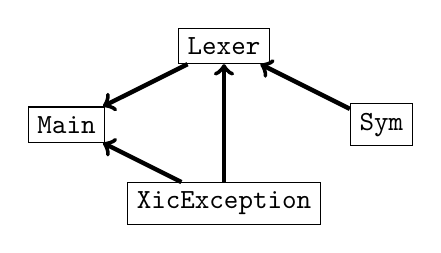
\begin{tikzpicture}
    \tikzstyle{every node}+=[draw]
    \node (main)  at (0, 0)  {\texttt{Main}};
    \node (lexer) at (2, 1)  {\texttt{Lexer}};
    \node (exn)   at (2, -1) {\texttt{XicException}};
    \node (sym)   at (4, 0)  {\texttt{Sym}};
    \path[->, ultra thick] (sym)   edge (lexer)
                           (exn)   edge (lexer)
                                   edge (main)
                           (lexer) edge (main);
  \end{tikzpicture}
  \caption{%
    Module Dependency Diagram. Each node represents a module. An arrow from
    module $u$ to module $v$ signifies that $v$ depends on $u$.
  }
  \label{fig:mdd}
\end{figure}

We had four main classes in our lexer, as shown in \figref{mdd}.
\begin{enumerate}
  \item{\texttt{Main}:}
    This is the main front end for our compiler. In this class, we handle the
    various command line options passed into the binary and call the rest of
    our lexing code. We also handle all IO (including the lexing analysis
    output) in this class.

  \item{\texttt{Lexer}:}
    This class is generated by JFlex from our lexer specification.  It is used
    to tokenize source Xi files.

  \item{\texttt{Sym}:}
    This class, generated by CUP, is our main internal representation of
    tokens.

  \item{\texttt{XicException}:}
    We subclass this abstract class to throw lexing errors (e.g.  empty
    characters) which we then handle internally.
\end{enumerate}

\subsection{Code Design}
One of the main extensions we implemented was in comments. The project
specification states that comments were only to be terminated by a newline, but
we allowed comments that were terminated by any line terminals (\verb$\r$,
\verb$\r\n$, and \verb$\n$) and by EOF.  We added the EOF case since it is
conceivable that programmers would end a source file with a comment, and having
a lexing failure in this case would be undesireable.

\newcommand{\minint}{9223372036854775808}
\newcommand{\maxint}{9223372036854775807}
Another design decisions revolved around the lexing of integer literals. In Xi,
integer literals fall in the range of $[-2^{63}, 2^{63}-1] = [-\minint,
\maxint]$. A peculiarity arises when lexing the string $s = $
\texttt{-\minint}. If a lexer parses $s$ as two tokens: a minus sign and an
integer literal, the integer literal $\minint$ is too large to be a valid
integer literal. This can be solved with regular expressions, though this
solution is inelegant. Instead, we introduce a new \texttt{BIG\_NUM} token
which is generated by the occurrence of \texttt{\minint}. We then defer the
responsibility of ensuring a \texttt{BIG\_INT} token is preceded by a minus
token to the parser.

We also added extensive lexical error support by way of our
\texttt{XicException} class. While the examples only gave the empty character
exception, we added several other error cases, such as out of bounds long
literals, invalid hex literals, unterminated strings and character literals,
and invalid tokens (a catch-all for symbols unsupported in the language
specification).

\subsection{Programming}
We implemented our lexer using both a bottom-up and a top-down approach. Some
members of our team used a bottom-up approach to implement our
\texttt{XicException} exception class and \texttt{Sym} symbol class---both
of which do not depend on any other class---without knowing exactly how they
would be used by other classes. Conversely, other members implemented our
\texttt{Main} class without yet knowing the specific implementation of the
underlying lexer. We also followed the designed principle of test driven
development, implementing tests cases as we implemented our lexer to catch bugs
often and early. This is described in detail in \secref{testing}.

We encountered various issues while implementing our lexer, most of which
revolved around the subtle interactions between whitespace characters and
regular expressions that are more complicated than they seem. The most
obnoxious issue revolved around the following regular expression we initially
used to match comments.

\begin{center}
\begin{BVerbatim}
LineTerminator = \n | \r | \r\n
Comment = "//" (!{LineTerminator})* {LineTerminator}
\end{BVerbatim}
\end{center}

Intuitively, the \texttt{Comment} regular expression matches \texttt{//}, any
number of characters that aren't \verb$\r$, \verb$\n$, or \verb$\r\n$, and
finally a line terminator. Surprisingly though, the string \verb$//a\r\na\n$ is
lexed as a single comment, not as a comment and then an identifier \verb$a$!
Inspecting the regular expression deeper, we see the language of
\verb${Comment}$ is \verb${\r, \n, \r\n}$. The language of \verb$!{Comment}$ is
then everything that's not in \verb${\r, \n, \r\n}$. This set includes
\verb$a\r$ and \verb$\na$! Thus, \verb$a\r\na$ is matched by
\verb$(!{LineTerminator})*$.

The distribution of work is described in detail in \secref{workplan}.

\section{Testing}\label{sec:testing}
We wrote numerous JUnit tests to verify the correctness of our lexer. We
started with very basic tests that would test one token at a time. Then, we
moved on to more complex tests where we would mix up different tokens or add
random white spaces before, after or between the tokens. After that we created
more test cases with escape characters, line terminators and EOF. Lastly, we
created invalid tests to make sure that we are throwing the correct exceptions.

Our test plan worked out very well. First testing on very basic tokens helped
us solidify the majority of our code. Then, testing with escape characters and
line terminators helped us find a lot of bugs in our code and made sure that we
were dealing with white spaces correctly.  Finally, testing that exceptions
were thrown properly again made sure we covered all the corner cases in our
lexer.

\section{Work Plan}\label{sec:workplan}
Before we started coding, one person set up the skeleton code and
modularization. Then another member took care of the frontend such as command
line interfaces. Then, other people wrote the rules for lexing while the other
members wrote test cases.

\section{Known Problems}\label{sec:problems}
None.

\section{Comments}\label{sec:comments}
We spent about 60 hours total on the assignment. The assignment overall
introduced important concepts about lexing but we thought the coding was a
little bit dry and tedious.

\end{document}
